\section{Alex Pitcher Report - Myles Denton}

\margininbox{Alex Pitcher, 2010}{As part of the funds coordinated by the Ghar Parau Foundation, ICCC received two Alex Pitcher memorial fund awards for Myles Denton and Kate Smith, who were both first year undergraduate students going on their first caving expedition. We reproduce Myles' report here.}{\award}


In July 2010, I was about to embark on my first caving expedition, at the end of a year's caving in the UK. It's easy to say that I was a little excited.


I have always been an adventurous person, I adore the outdoors and I have a great interest in the
Earth and thus joining ICCC in October was the inevitable outcome! I had never been caving before,
and from the initial presentations and meetings, I was extremely keen to get below-ground. Soon
enough, I was hooked and was looking forward to heading off on a 4 week expedition to the Julian
Alps in Slovenia.


Slovenia was one of the hardest and most rewarding experiences I have had. After packing up
a month's worth of supplies and cramming as much of it into the minibus as possible, our group of
intrepid cavers set off towards Slovenia, a journey taking us through six countries over twenty four
hours.


\begin{pagefigure}
\checkoddpage \ifoddpage \forcerectofloat \else \forceversofloat \fi
   \centering
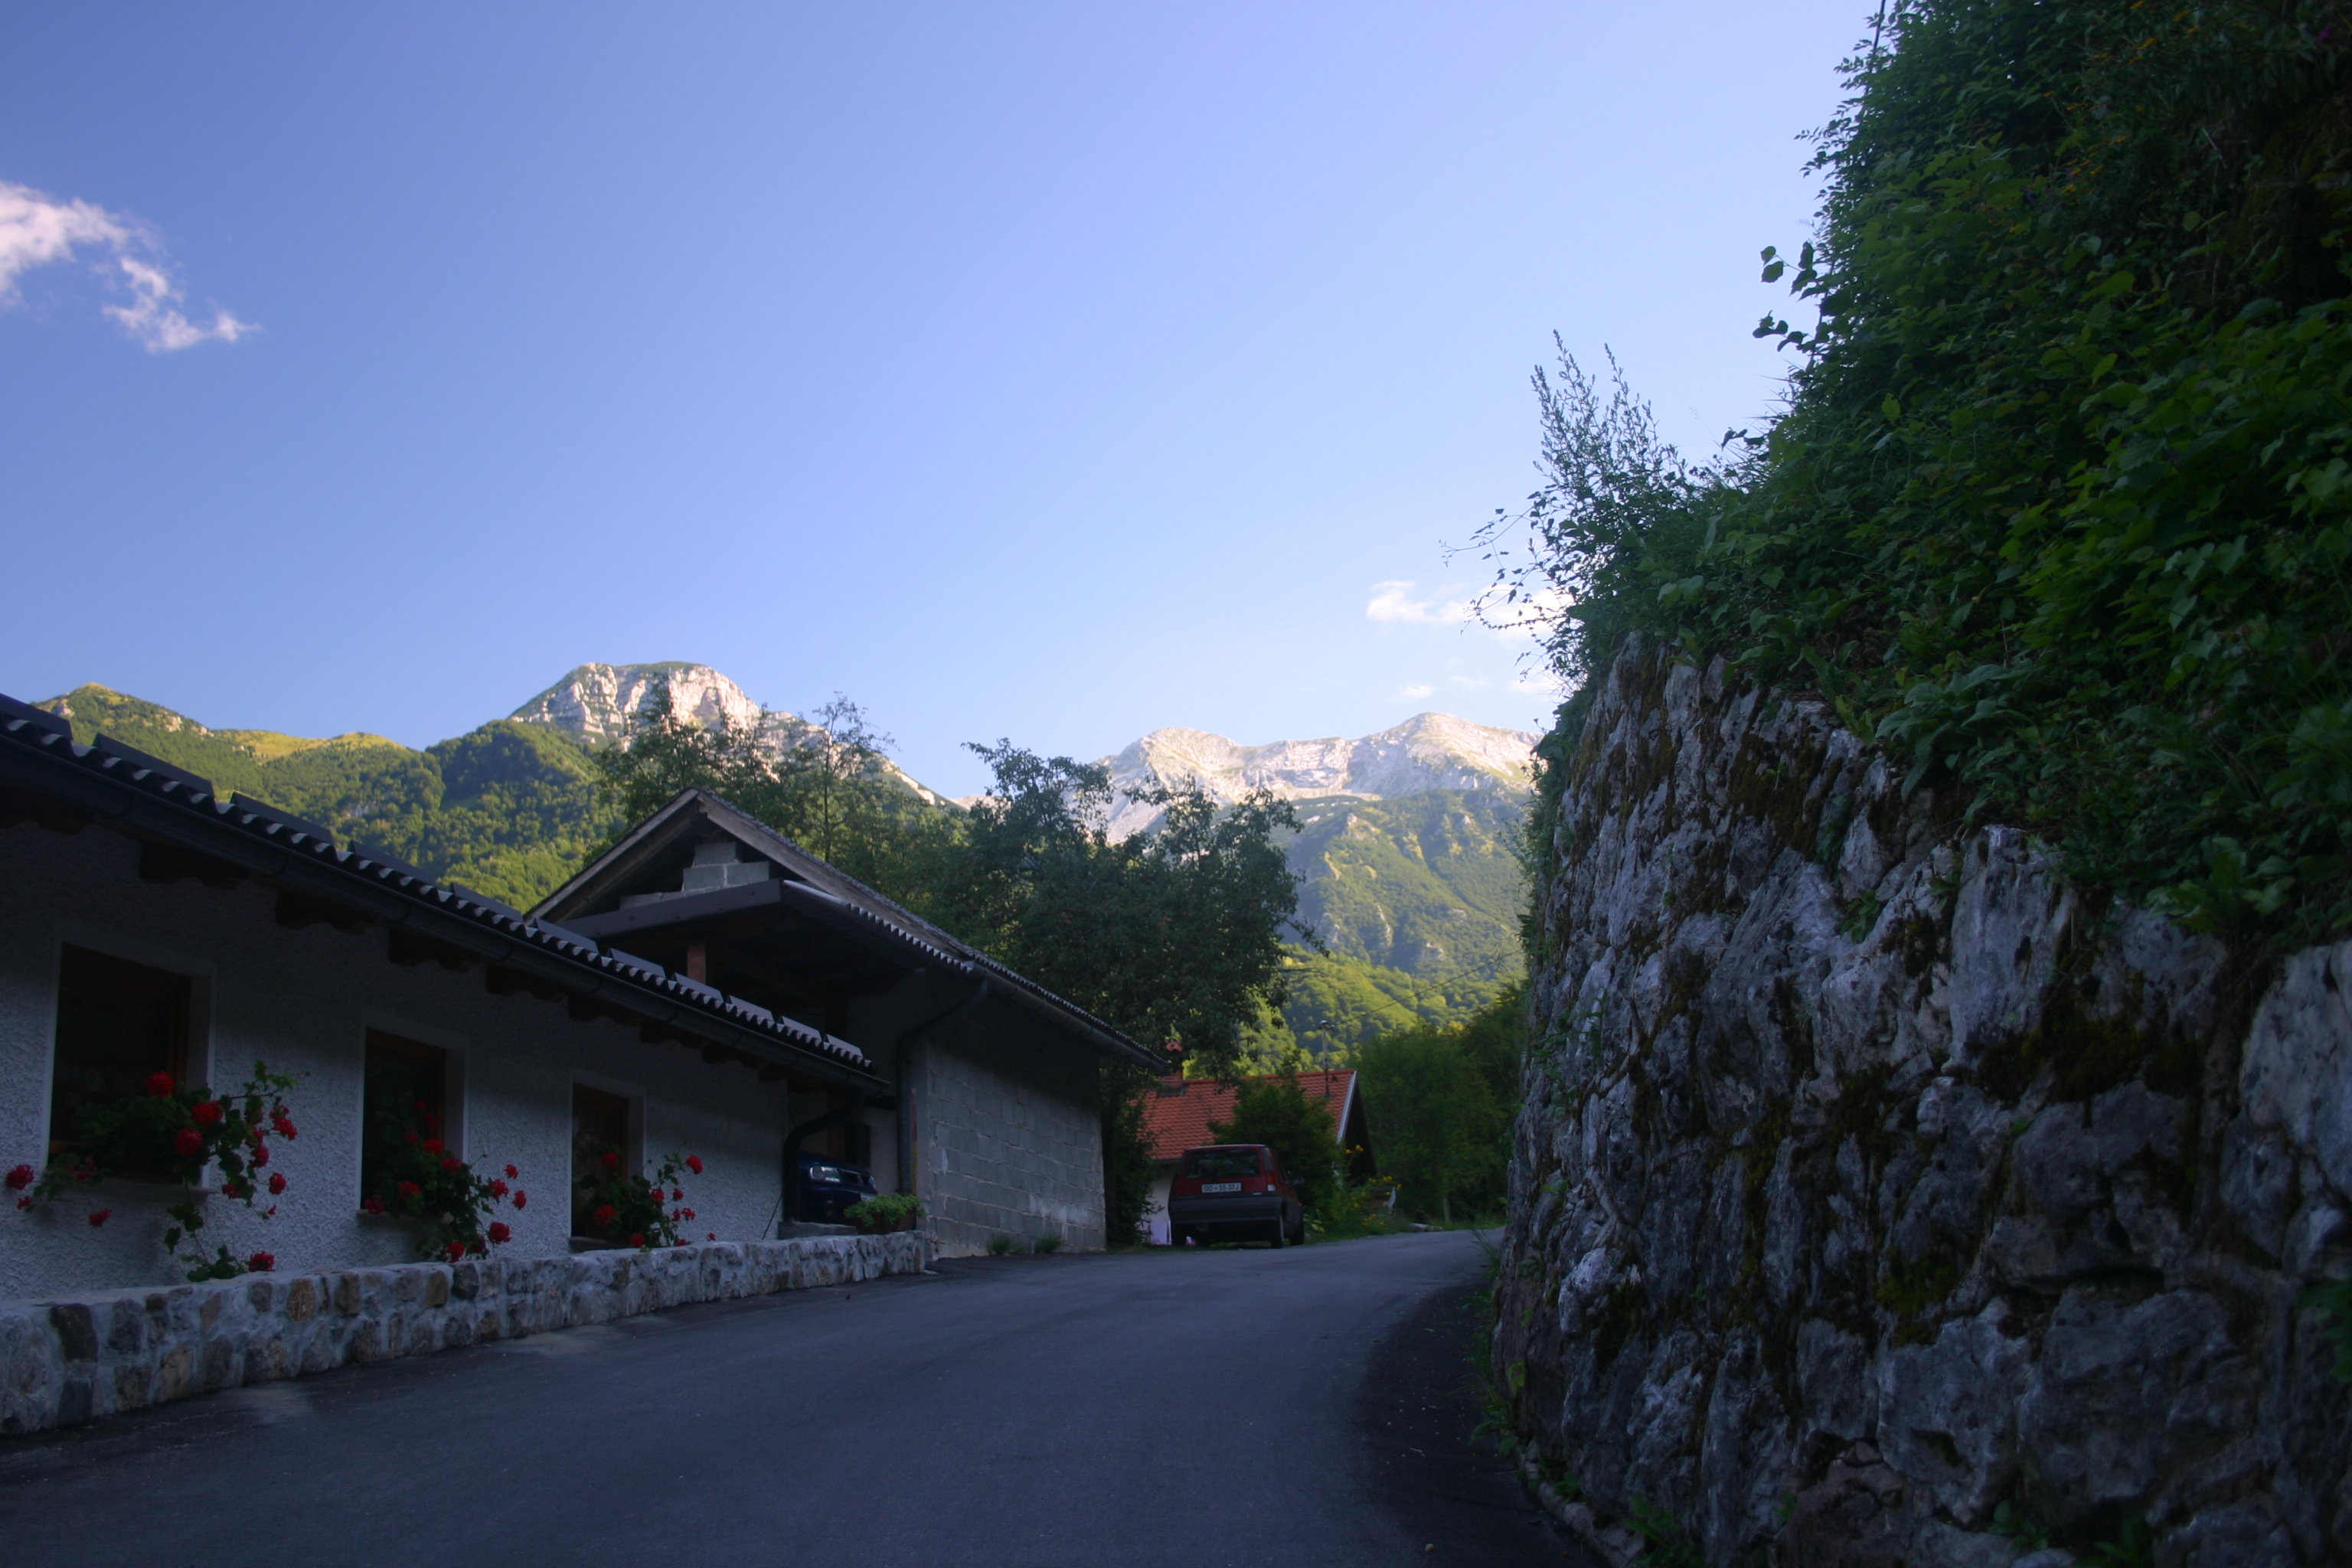
\includegraphics[width = \textwidth]{2010/expo_stories/20100731-14-22-42 - Tharatorn Supasiti - IMG_6366 --orig.jpg}
\caption{\protect\passage[mountain]{Tolminski Migovec} is prominent on the horizon as one leaves \protect\passage[town]{Tolmin} and takes the road to \protect\passage[town]{Tolminske Ravne}. \pic{Tharatorn Supasiti}} \label{leaving tolmin}
\end{pagefigure}

Arriving in Slovenia I was immediately taken aback by the country's beauty, and after spending
a night eating pizza and sleeping in \passage[town]{Tolmin}, we began our ascent of \passage[mountain]{Migovec}. The mountain plateau
where our base camp was set up is at an altitude between 1800m and 2000m. Driving to a farm at
\passage[town]{Ravne}, we shared coffee, packed any remaining space in our bags with food, and headed up \passage[mountain]{Migovec}.
The first trip to the top was accompanied by a rain cloud, which left us wet, but nicely cool up to the
top. The next few days were taken up by cavers making trips up and down the mountain, ferrying
equipment, food and most importantly huge volumes of very heavy cheese!


\begin{figure*}[t!]
\checkoddpage \ifoddpage \forcerectofloat \else \forceversofloat \fi
\frame{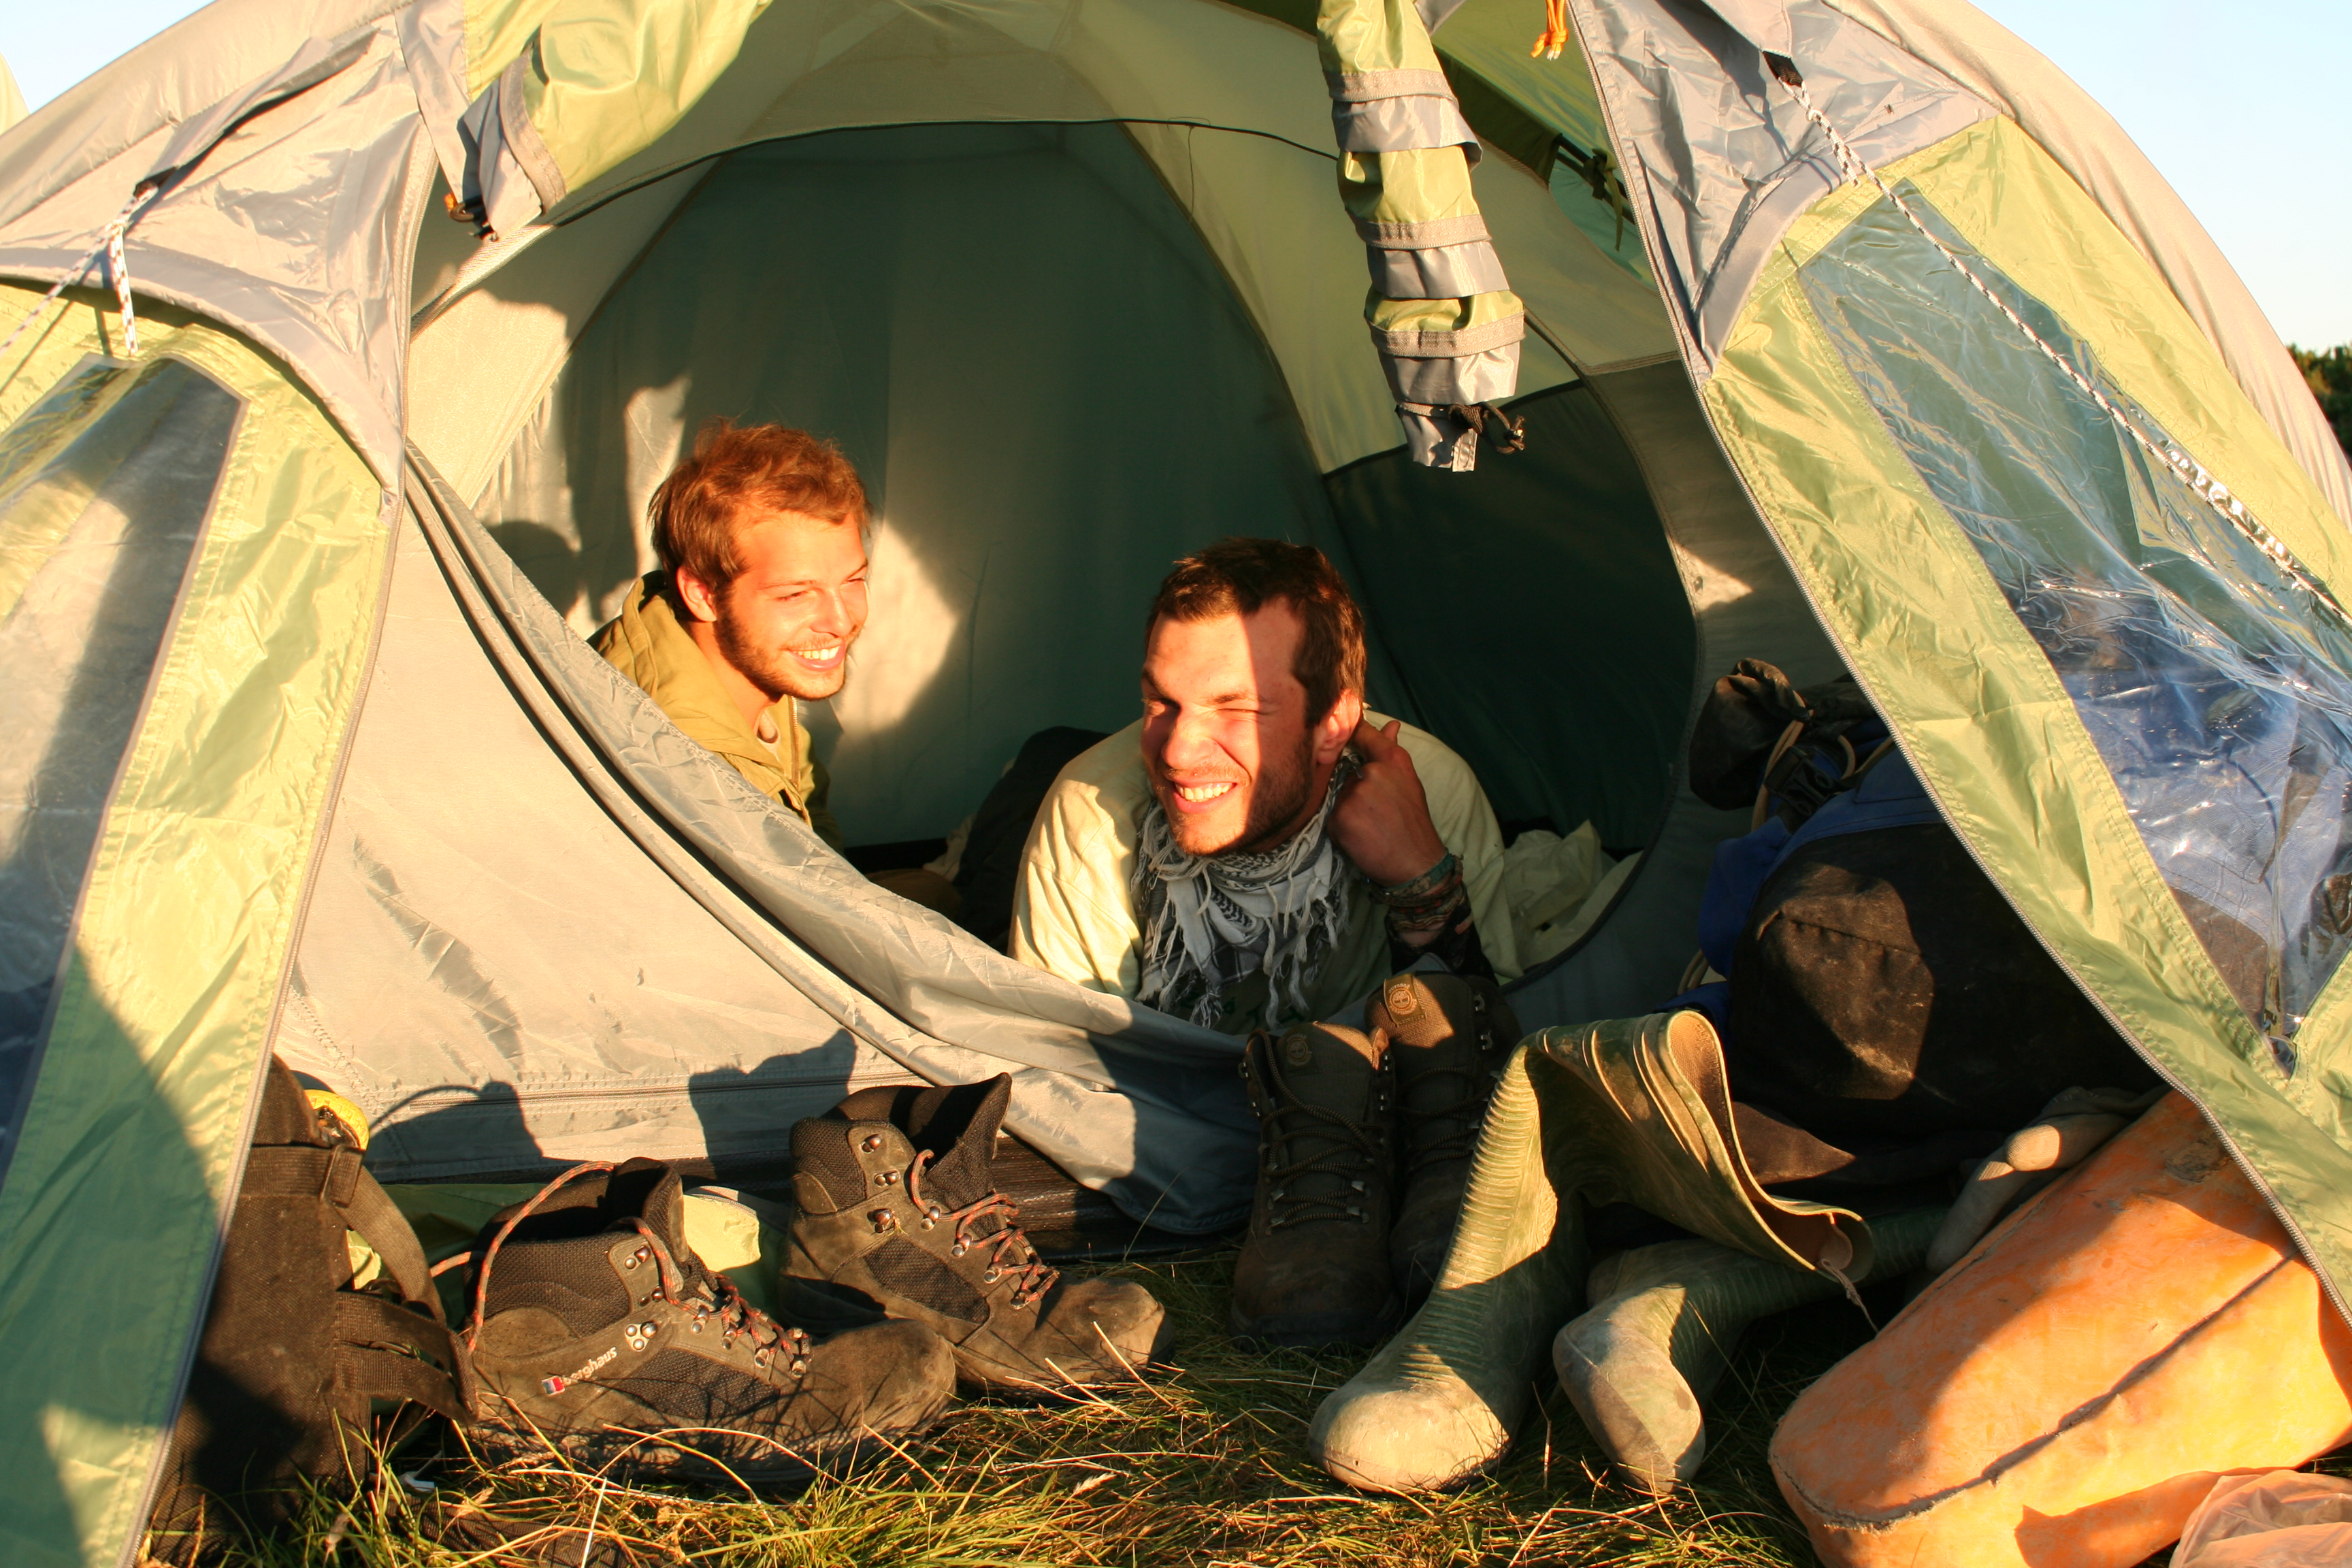
\includegraphics[width=\linewidth]{2010/ap_awards/20100803-18-10-06 - Jana Carga 09--orig.jpg}}
\caption{The evening sun shining on Myles and Niko. \pic{Jana Čarga}}
\end{figure*}





After being showed around the plateau, introduced to the various cave entrances and schooled on
the history of the caving on the mountain Nikolas Kral and I prepared for our first sortie underground,
with experienced caver James "Tetley" Hooper. Our first trip was in the \passage{Vrtnarija} cave system.
Descending through the entrance dubbed \passage{Gardeners' World}, the three of us made a steady descent to
the bottom of the \passage{Pico} pitch, at about -200 m. This was already deeper than either of us had been
in our nine month caving experience in the UK!


\margininbox{23-7 10:30pm}{

Fucking body won't fall asleep! Must have only had a couple of hours at
most since Dan arrived. [...] Tetley's bodily functions are out of
control! May bring some corks down for his digestive tract next time.
Anyway, now for some food and tea and hopefully can stay awake till
bedtime at noon! \name{Myles Denton}}{\logbook}


The following day, infested by the caving bug, Tetley
and I again entered \passage{Vrtnarija}, this time descending to the top of \passage{Fistful of Tolars} pitch, at -400 m.
These trips also doubled up as opportunities to take some of the gear needed to set up camp at -550
m. Several other caving trips were made, taking the nine tackle bags down to the middle of \passage{Friendship
Gallery}. These included Kate Smith, another fresher, on her first expedition with Nick and I.


The cave system within \passage{Migovec} is genuinely breath taking. Whilst not the most decorated of caves
(which we later discover not to be true), the sheer nature of the cave is beautiful. Descending through
large chambers, with pitches up to 120 m, is an exhilarating experience, learning to slide through those
tricky parts of the cave and strolling through the large phreatic passages is incredibly liberating.






\fullwidthbox{Pushing \passage{Black Knight}}{

\textit{28-7 12:55}\\
Another 7 bolts added to \passage{Black Knight} pitch at end of \passage{Korita}. Once down the stream flowed into a duck. “There will be a bypass” I declared\ldots{} and there was! The stream passage continued – we stayed high. Eventually $\approx$15m drop to stream. But Myles found a dry passage – strongly draughting – that goes to a $\approx$10m pitch. This dry route we called \passage{Sidewinder}. 130m in survey book. We left $\approx$25m of 9mm rope at bottom of \passage{Black Knight} – nothing else left there. James and Jan are somewhere down \passage{Big Rock} – hope they’re OK\ldots{}
\name{Tetley}

\textit{28-7 1pm}\\
Returned from this storming push with Tetley. We now have two pretty beastly leads. Was a bit tired during final rigging of \passage{Black Knight} but perked up as soon as we found new passage. Now in underground camp. Thought we’d killed it all when we found the duck but Tetley saved us with his bypass seeking skills. Had to heat up Nick’s willies[sic] over the gas stove until they were flexible enough to fit on his clodhoppers. Him and Gergely are off to push now.
\name{Myles}}


\margininbox{Black Knight}{
     \begin{itemize}
    \item Myles Denton
    \item James "Tetley" Hooper
    \end{itemize}}{\explo}



\begin{marginfigure}
\checkoddpage \ifoddpage \forcerectofloat \else \forceversofloat \fi
\centering
 \frame{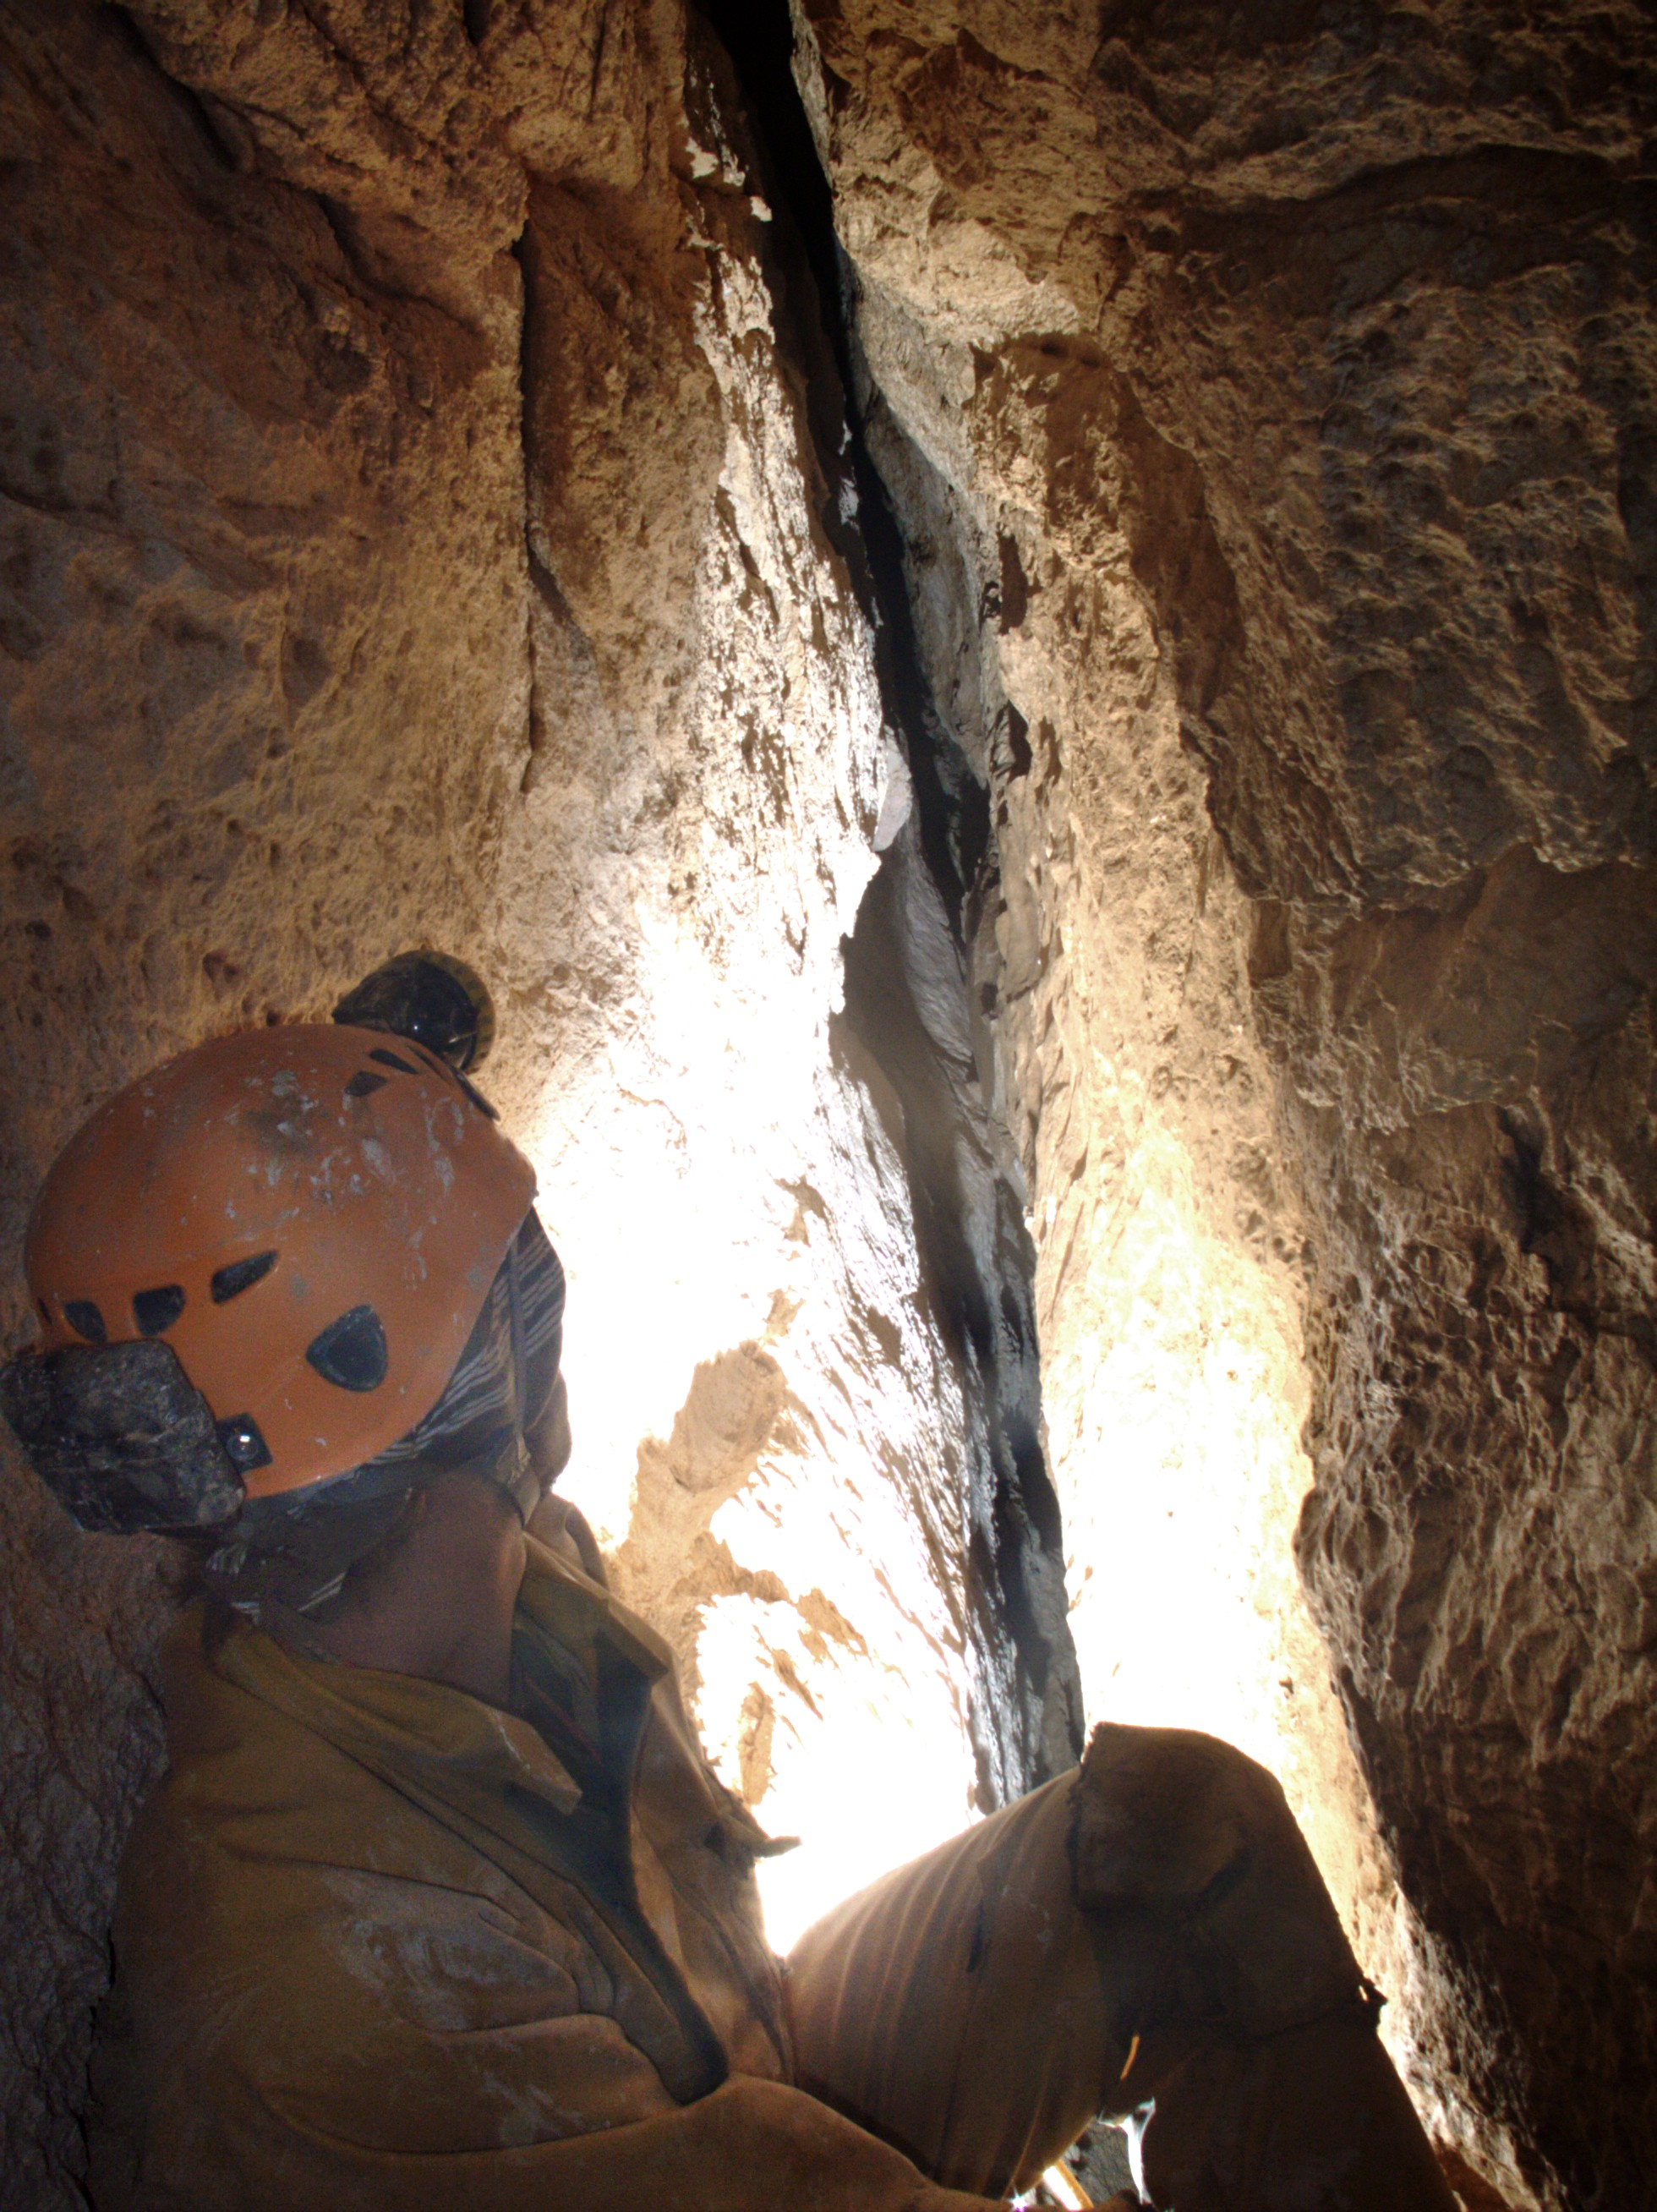
\includegraphics[width=\linewidth]{2010/ap_awards/20100806-16-24-30-Jarvist Frost-Canon G5-CRW_0479-Myles Stalemate end of Tolminksa Korita--orig.jpg}} 
 \caption{Myles looking down the impassable rift at the end of \protect\passage{Stalemate}, one of the only two people to see this place in real life. \pic{Jarvist Frost}}
 \label{stalemate rift}
\end{marginfigure}


Soon enough, I was ready to head to Camp \passage{X-Ray}, our underground camp at -550 m. Our underground camp consisted of a 4 man single layer tent, which helped to raise the temperature of 1$^{\circ}$C by a few degrees. We had two Vango Nitestar 450 sleeping bags, which are brilliant, and a set of
two buffalo bags, which enabled our camp to become a four man camp. We used methylated spirits
and gas stoves to cook with, and had several candles for ambience! As well as a first aid kit, we had
a small set of speakers, a small video system and an mp3 full of Blackadder. At -550 m, all this made
underground camp a very welcome place indeed.


On my first trip to underground camp Tetley and I spent one night there, pushing the \passage{Tolminska
Korita} series for several hours, and discovering the pitch later named \passage{Black Knight}. We were joined
by Gergely and Andy after our stay at underground camp, who informed us they'd been pushing a
messy pitch named \passage{Leopard}, which had burst into a decorative horizontal passage which had many
leads. We were all excited. On the surface, I helped input our survey data into the computer, and
reviewed the new passage we had discovered.


Over the next week or so, several caving parties went below, mainly pushing the \passage{Leopard} series.
Tetley and I returned to push \passage{Black Knight}, which entered further pitches, and then hit a duck. Here I was worried the passage was blocked by the water, however, Tetley cunningly discovered a bypass
passage which passed over and around the duck. Jana Čarga and Jarvist Moore Frost pushed the series
and closed on part, \passage{Sidewinder}, as it dropped into a part of the cave known as \passage{Envy}, at about -660 m.
On my last pushing trip towards the end of expedition, Jarvist and I closed the final part of the \passage{Black Knight} series, named \passage{Stalemate}, where the water flowed into a narrow rift too small for us to squeeze through despite our attempts.


\begin{figure*}[t!]
\checkoddpage \ifoddpage \forcerectofloat \else \forceversofloat \fi
\frame{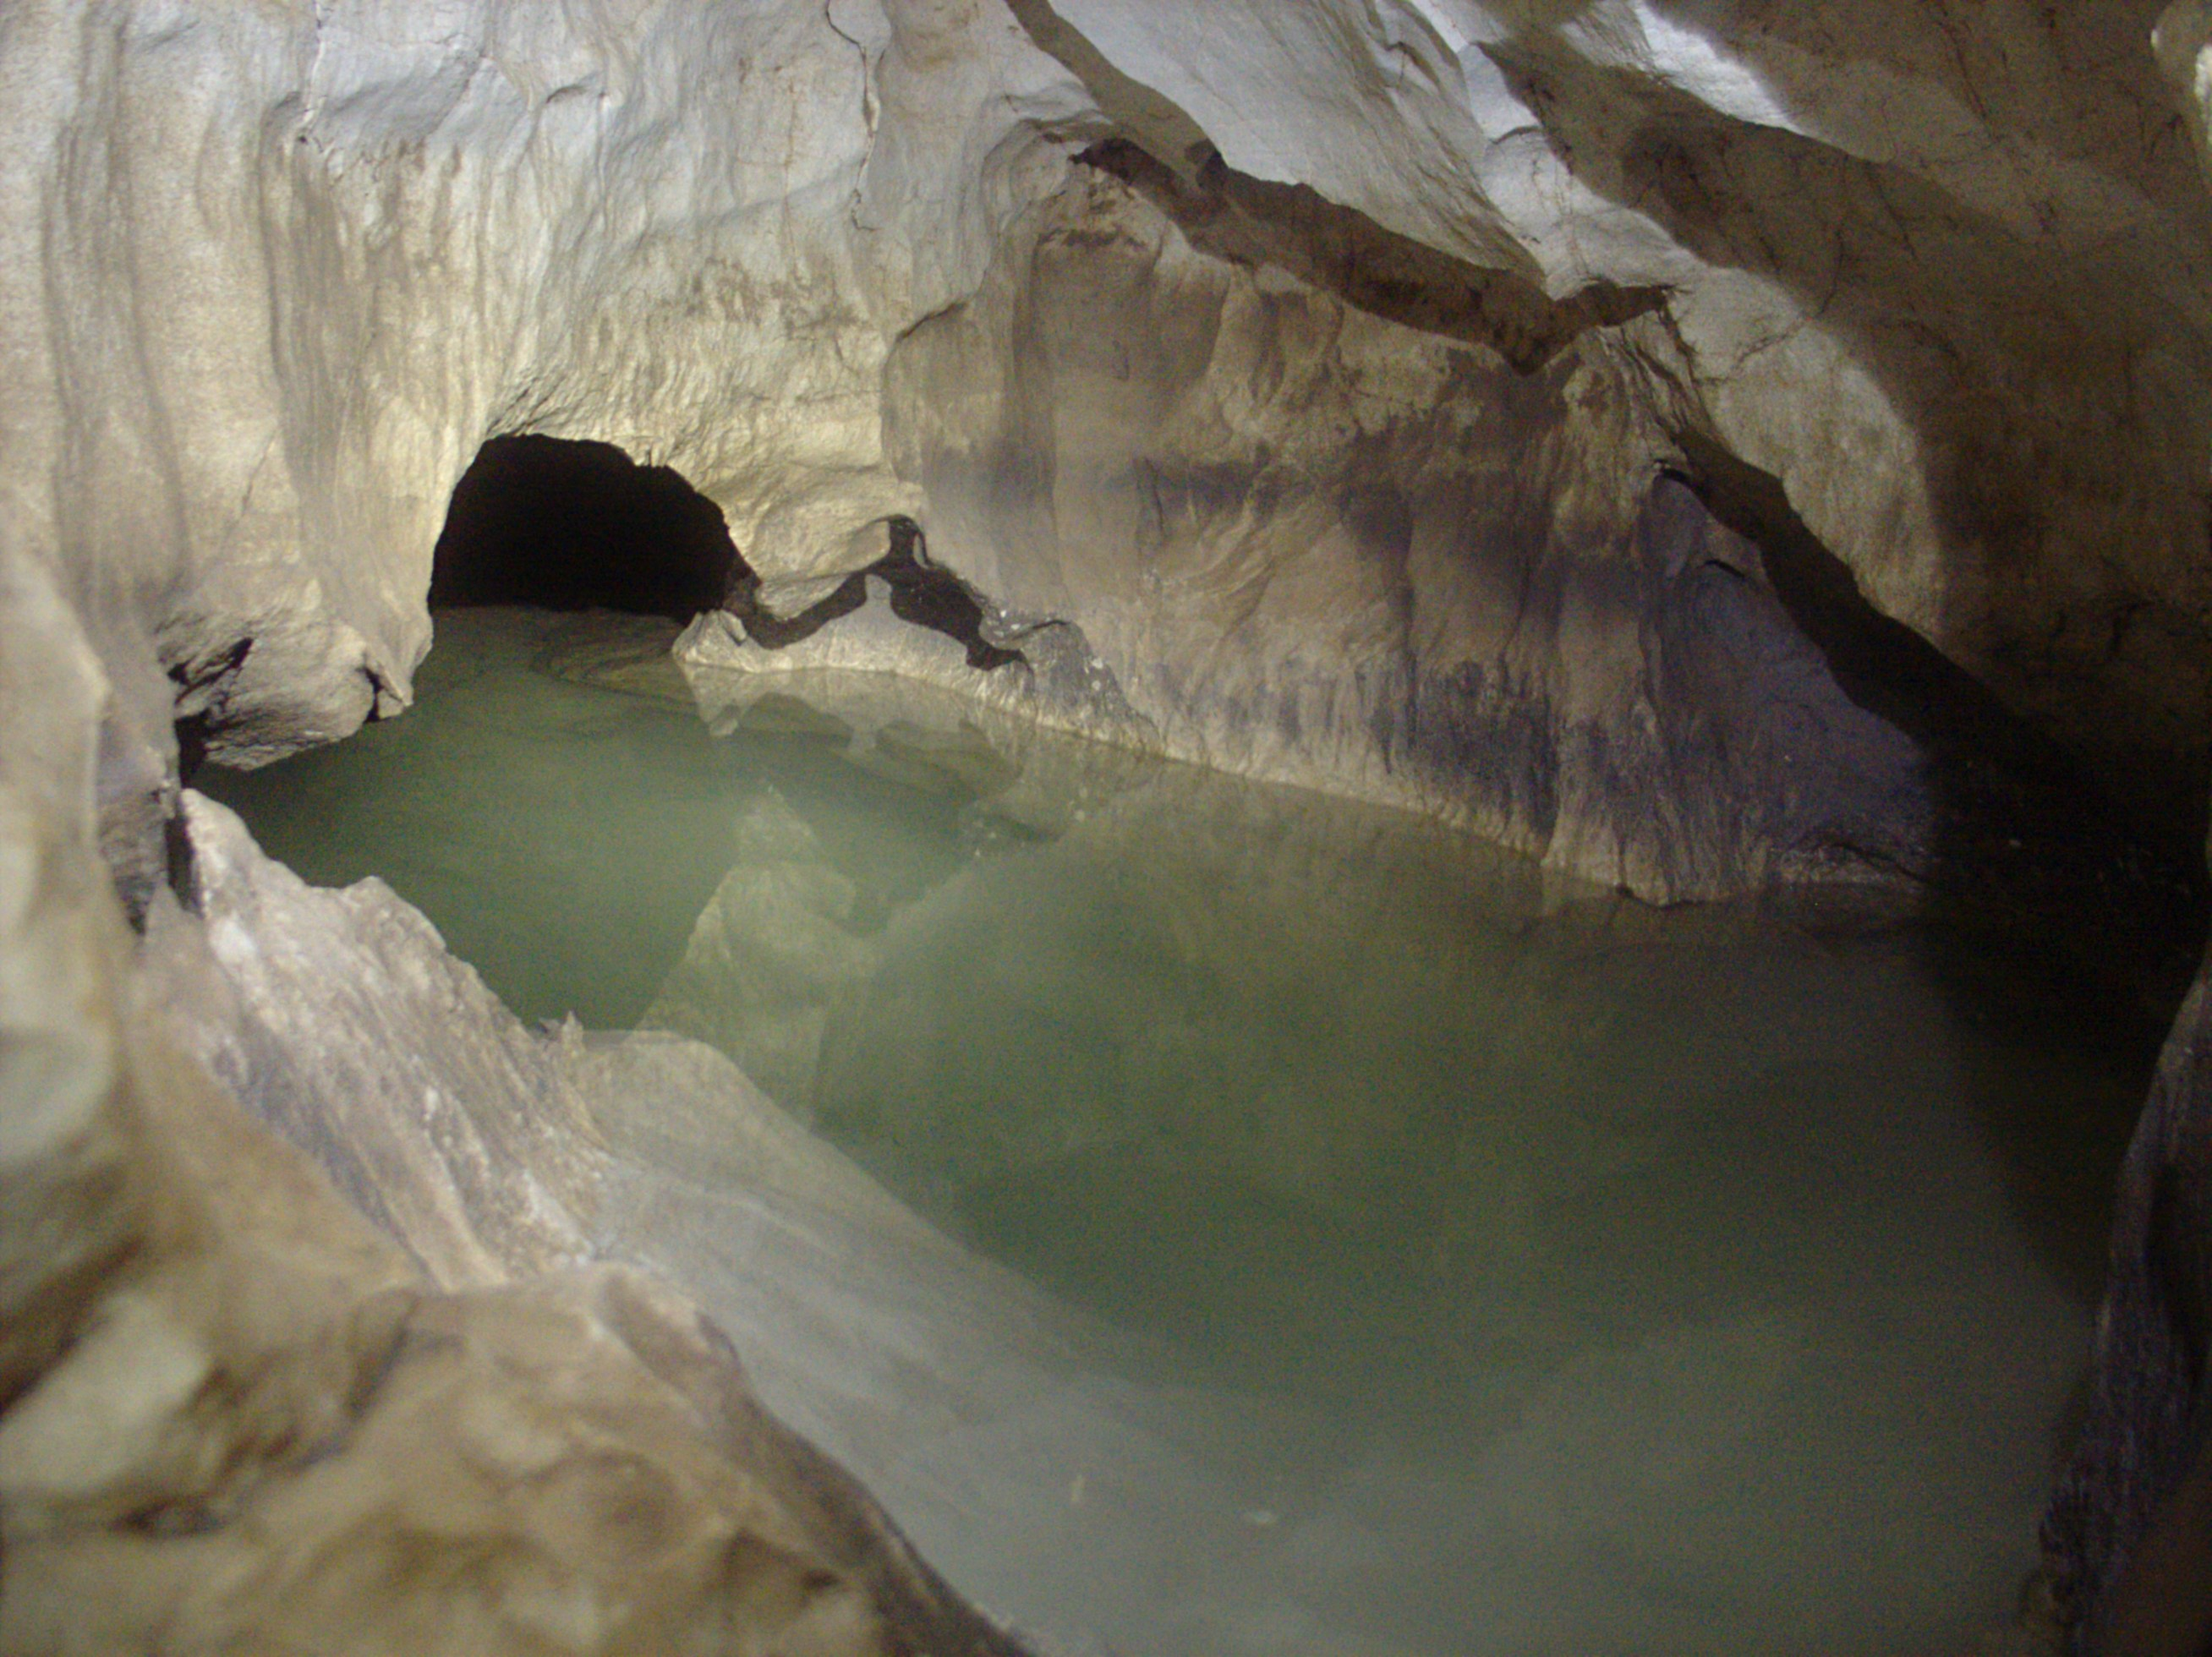
\includegraphics[width=\linewidth]{2010/ap_awards/20100801-16-44-48-Jarvist Frost-Canon G5-CRW_0420-colour-Black Knight bypassed duck--orig.jpg}}
\caption{The far side of the duck in the \passage{Black Knight} series. A bypass on the near side was quickly discovered, enabling continuing exploration to the passages \passage{Sidewinder} and \passage{White Bishop}. \pic{Jarvist Frost}}
\end{figure*}


Overall, my Slovenian expedition was life changing. 2.2 km of undiscovered cave was found, between about twenty cavers. Personally I discovered around 310 m of passage with my partners. More
importantly, my caving skills improved hugely: I went from taking 3 hours to get to -550m to 1 hour
45 minutes; I learnt how to install bolts; how to tie many knots, and where to use them. My techniques
for both abseiling and prussiking improved greatly, and overall I became more confident and proficient
in all aspects of caving. I don't think twice about hauling several tackle bags down a cave anymore!
The funding from Alex Pitcher helped me to purchase a Petzl helmet and Mig light\sidenote{the original name of Dave Wilson's design of helmet-mounted caving light, renamed later as 'Bisun' lights} attachment, which I used on every underground trip.

\name{Myles Denton}
